% ============================================================================
%  main.tex — Universal LaTeX Template (Entry Point)
%  Author:  Yazid TAHIRI ALAOUI
%  Usage:   Edit the metadata commands below, then compile with pdflatex.
% ============================================================================
\documentclass[a4paper,12pt]{report}

% ── Load the style package ──────────────────────────────────────────────────
\usepackage{styles/yazid-template}

% ============================================================================
%  DOCUMENT METADATA  — Edit these for each new project
% ============================================================================
\newcommand{\docKingdom}{ROYAUME DU MAROC}
\newcommand{\docUniversity}{Université Abdelmalek Essaâdi}
\newcommand{\docSchool}{École Nationale des Sciences Appliquées d'Al Hoceima}
\newcommand{\docTitle}{Implémentation d'une architecture Kappa}
\newcommand{\docSubtitle}{Traitement événementiel unifié pour le e-commerce}
\newcommand{\docModule}{Gestion de Projets Informatiques}
\newcommand{\docAuthor}{Yazid TAHIRI ALAOUI, Souhayla ECH-CHARAY et Ouissal EL AMRANI}
\newcommand{\docProgram}{1\`{e}re année -- Ingénierie Données (ID1)}
\newcommand{\docSupervisor}{Pr. Redouan ABAKOUY}
\newcommand{\docYear}{2025 -- 2026}

% ── Headers (uses commands from the .sty) ───────────────────────────────────
\renewcommand{\headerLeft}{Projet Architecture Kappa}
\renewcommand{\headerRight}{ENSAH -- Année 2025/2026}

% ── PDF metadata ────────────────────────────────────────────────────────────
\hypersetup{
    pdftitle={\docTitle},
    pdfauthor={\docAuthor},
    pdfsubject={\docModule},
    pdfkeywords={Architecture Kappa, Kafka, Traitement de flux, E-commerce, Gestion de projet}
}

% ============================================================================
%  BEGIN DOCUMENT
% ============================================================================
\begin{document}

% ── Title Page ──────────────────────────────────────────────────────────────
% ============================================================================
%  titlepage.tex — Parameterised Title Page
%  Uses TikZ decorative border + mdframed author box
%  All values come from \newcommand definitions in main.tex
% ============================================================================

\begin{titlepage}
    % --- Decorative double border ---
    \begin{tikzpicture}[remember picture, overlay]
        \draw[primarycolor, line width=2.5pt]
            ($(current page.north west) + (1.2cm,-1.2cm)$)
            rectangle
            ($(current page.south east) + (-1.2cm,1.2cm)$);
        \draw[accentcolor, line width=0.8pt]
            ($(current page.north west) + (1.4cm,-1.4cm)$)
            rectangle
            ($(current page.south east) + (-1.4cm,1.4cm)$);
    \end{tikzpicture}

    \vspace*{0.5cm}

    % --- Institutional logos ---
    % Place your logos in the logos/ folder and adjust filenames / widths
    \begin{minipage}{0.3\textwidth}
        
\includegraphics[width=3.5cm]{logos/UAE.png}
    \end{minipage}
    \hfill
    \begin{minipage}{0.3\textwidth}
        \raggedleft
        
\includegraphics[width=2cm]{logos/ENSAH.png}
    \end{minipage}

    \vspace*{1cm}

    \begin{center}
        % --- Institution lines ---
        {\large \textbf{\textcolor{primarycolor}{\docKingdom}}}\\[0.3cm]
        {\large \textbf{\docUniversity}}\\[0.3cm]
        {\large \textbf{\docSchool}}\\[2.5cm]

        % --- Title block ---
        \textcolor{accentcolor}{\rule{0.8\linewidth}{1.5pt}}\\[0.4cm]
        {\huge\textbf{\textcolor{primarycolor}{\docTitle}}}\\[0.5cm]
        {\LARGE\textbf{\docSubtitle}}\\[0.3cm]
        \textcolor{accentcolor}{\rule{0.6\linewidth}{1.5pt}}\\[0.6cm]

        % --- Module / course line ---
        {\large \textbf{\textit{\docModule}}}\\[0.2cm]

        \vspace{2.5cm}

        % --- Author information box ---
        \begin{mdframed}[linecolor=accentcolor, linewidth=1pt, roundcorner=10pt,
            backgroundcolor=white, userdefinedwidth=0.8\textwidth, align=center]
            \centering
            \vspace{0.3cm}
            \large\textbf{\textcolor{primarycolor}{Réalisé par :}}\\[0.2cm]
            \textbf{\docAuthor}\\[0.4cm]
            \large\textbf{\textcolor{primarycolor}{Filière :}} \docProgram\\[0.2cm]
            \large\textbf{\textcolor{primarycolor}{Encadré par :}} \docSupervisor\\
            \vspace{0.3cm}
        \end{mdframed}

        \vfill
        {\large \textbf{\textcolor{primarycolor}{Année universitaire : \docYear}}}
    \end{center}
    \vspace*{0.5cm}
\end{titlepage}


% ── Front Matter (roman page numbers) ──────────────────────────────────────
\pagenumbering{roman}
\newgeometry{left=2.5cm, right=2.5cm, top=2.5cm, bottom=2.5cm, headheight=15pt}

% ── Abstract / Résumé ──────────────────────────────────────────────────────
\renewcommand{\thechapter}{\Roman{chapter}}
% ============================================================================
%  abstract.tex — Résumé / Abstract Template
%  Replace the placeholder text below with your project's summary.
% ============================================================================

% --- French Abstract ---
\chapter*{Résumé}
\addcontentsline{toc}{chapter}{Résumé}

\vspace{0.5cm}

Dans le cadre du module de \textbf{Gestion de Projets Informatiques} dispensé à l'École Nationale des Sciences Appliquées d'Al Hoceima, ce projet vise à concevoir, implémenter et valider une \textbf{architecture Kappa} appliquée à une plateforme e-commerce fictive.

\vspace{0.3cm}

Face à la complexité croissante des architectures de données traditionnelles --- notamment l'architecture \textbf{Lambda} qui impose la maintenance de deux couches distinctes de traitement (batch et temps réel) ---, l'architecture \textbf{Kappa}, proposée par Jay Kreps en 2014, offre une alternative élégante reposant sur un \textbf{unique flux de traitement continu}. Ce projet démontre concrètement cette approche en déployant une infrastructure complète composée d'\textbf{Apache Kafka} (log d'événements), \textbf{Apache Flink} (référence de traitement de flux) et \textbf{Docker} (conteneurisation).

\vspace{0.3cm}

Le système mis en place traite en temps réel des événements comportementaux simulés (vues, ajouts au panier, achats, abandons) à travers trois topologies spécialisées : le \textbf{filtrage des bots}, l'\textbf{agrégation statistique par fenêtres temporelles} et la \textbf{détection d'abandon de panier} avec alertes marketing. La validation du système repose sur le mécanisme de \textbf{replay} --- pierre angulaire de l'architecture Kappa --- qui permet de rejouer l'intégralité du journal d'événements pour recalculer les résultats et confirmer leur parfaite cohérence avec le traitement temps réel.

\vspace{0.3cm}

Le projet a été conduit selon une méthodologie \textbf{Agile (Scrum + Kanban)}, structuré en 4 sprints, avec une gestion rigoureuse des risques et une planification par \textbf{Planning Poker}. L'ensemble du processus a été suivi via \textbf{Taiga} (Kanban) et \textbf{GanttProject} (planification temporelle).

\vspace{0.5cm}

\noindent\textbf{Mots-clés :} Architecture Kappa, Apache Kafka, Traitement de flux, Temps réel, E-commerce, Rétention, Replay, Docker, Gestion de projet Agile.

\vfill


% ── Table of Contents ──────────────────────────────────────────────────────
\newpage
\renewcommand{\contentsname}{Table des matières}
\tableofcontents
\newpage

% ── List of Figures ────────────────────────────────────────────────────────
\renewcommand{\listfigurename}{Liste des figures}
\listoffigures
\newpage

% ── List of Tables ─────────────────────────────────────────────────────────
\renewcommand{\listtablename}{Liste des tableaux}
\listoftables
\newpage

% ── Main Content (arabic page numbers) ─────────────────────────────────────
\pagenumbering{arabic}
\setcounter{page}{1}
\renewcommand{\thechapter}{\arabic{chapter}}
\setcounter{chapter}{0}

% ── Include your chapters here ─────────────────────────────────────────────
\chapter{Introduction : Architecture Kappa}

\section{Contexte et Objectifs}

Le présent projet s'inscrit dans le cadre du module de \textbf{Gestion de Projets Informatiques} (Pr. Abakouy --- ENSA Al Hoceima) et vise à concevoir une architecture de traitement événementiel unifié pour une plateforme e-commerce fictive. L'objectif principal est de remplacer l'architecture classique Lambda par une \textbf{architecture Kappa}, proposée par \textbf{Jay Kreps} (co-créateur d'Apache Kafka) en 2014.

\begin{infobox}
    \centering
    \vspace{0.3cm}
    {\large \textbf{Principe fondamental de Kappa :} Un \textit{unique flux de traitement continu} pour toutes les données, qu'elles soient en temps réel ou historiques.}
    \vspace{0.3cm}
\end{infobox}

\section{Architecture Lambda vs Kappa}

L'architecture \textbf{Lambda} (2011, Nathan Marz) sépare le traitement en deux couches distinctes : une couche \textit{batch} (retraitement périodique via MapReduce ou Spark) et une couche \textit{speed} (traitement temps réel via Storm ou Flink). Cette séparation engendre une complexité opérationnelle considérable et une duplication du code métier.

L'architecture \textbf{Kappa} (2014, Jay Kreps) repose, en revanche, sur un unique flux de traitement continu. Toutes les données sont traitées par le même système. La rétention des événements dans un log distribué (Apache Kafka) permet de recalculer n'importe quel résultat en rejouant simplement le flux depuis le début (\textit{Replay}).

\begin{table}[H]
\centering
\begin{tabularx}{\textwidth}{L{3.5cm} C{3.5cm} C{3.5cm} C{3cm}}
\toprule
\textbf{\color{primarycolor}Critère} &
\textbf{\color{primarycolor}Lambda} &
\textbf{\color{primarycolor}Kappa} &
\textbf{\color{primarycolor}Notre choix} \\
\midrule
Temps réel & Oui & Oui & \textbf{Kappa} \\
\addlinespace[0.1cm]
Simplicité & 2 systèmes & 1 système & \textbf{Kappa} \\
\addlinespace[0.1cm]
Cohérence & Merge complexe & Replay natif & \textbf{Kappa} \\
\addlinespace[0.1cm]
Replay & Batch séparé & Natif Kafka & \textbf{Kappa} \\
\addlinespace[0.1cm]
Coût opérationnel & Élevé & Réduit & \textbf{Kappa} \\
\bottomrule
\end{tabularx}
\caption{Comparaison des architectures Lambda et Kappa}
\end{table}

\section{Les Trois Piliers de l'Architecture Kappa}

\subsection{Pilier 1 : Le Log d'Événements (Kafka)}
Tous les événements sont stockés de manière \textbf{immuable} et \textbf{ordonnée} dans Apache Kafka. La \textit{rétention} définit combien de temps les événements sont conservés. Ce log permet le \textit{replay} : relire l'historique depuis n'importe quel point dans le temps.

\subsection{Pilier 2 : Le Traitement de Flux (Topologies)}
Les événements sont traités \textbf{en continu} par des topologies spécialisées. Chaque topologie a une responsabilité unique (filtrage, agrégation, détection de patterns). Les topologies forment une \textit{chaîne de traitement} (pipeline).

\subsection{Pilier 3 : Le Replay pour la Cohérence}
Lorsque la logique de traitement change, on déploie une nouvelle version de la topologie. Celle-ci \textit{rejoue} tous les événements depuis le début du log. Le résultat est \textbf{identique} à ce qu'aurait produit un batch layer classique, sans la complexité associée.

\section{Pourquoi Kappa pour le E-commerce ?}

Pour une plateforme e-commerce, les événements comportementaux (clics, paniers, achats) sont \textbf{naturellement des flux}. L'architecture Kappa est parfaitement adaptée car :

\begin{enumerate}
    \item Les données arrivent \textbf{en continu} (les clients naviguent en permanence) ;
    \item On a besoin de \textbf{réactivité} (détecter un abandon de panier immédiatement) ;
    \item On veut pouvoir \textbf{recalculer} les statistiques si la logique métier change.
\end{enumerate}

\section{Technologies Utilisées}

\begin{table}[H]
\centering
\begin{tabularx}{\textwidth}{L{3.5cm} X C{2.5cm}}
\toprule
\textbf{\color{primarycolor}Technologie} &
\textbf{\color{primarycolor}Rôle} &
\textbf{\color{primarycolor}Version} \\
\midrule
Apache Kafka & Log d'événements, rétention, distribution & 7.3.0 (Confluent) \\
\addlinespace[0.1cm]
Apache Zookeeper & Coordination du cluster Kafka & 7.3.0 (Confluent) \\
\addlinespace[0.1cm]
Apache Flink & Moteur de traitement de flux (référence) & 1.17 \\
\addlinespace[0.1cm]
Python & Scripts de simulation et topologies & 3.10+ \\
\addlinespace[0.1cm]
kafka-python & Client Python pour Kafka & 2.3.x \\
\addlinespace[0.1cm]
Docker & Conteneurisation de l'infrastructure & 29.x \\
\addlinespace[0.1cm]
Docker Compose & Orchestration des services & 5.x \\
\bottomrule
\end{tabularx}
\caption{Stack technologique du projet}
\end{table}

\chapter{Acteurs et Rôles}

\section{Gouvernance du Projet}

Conformément aux principes de gestion de projet (Chapitre 2 du cours), nous avons identifié les parties prenantes selon le modèle classique \textbf{MOA / MOE / Chef de Projet}.

\subsection{Maîtrise d'Ouvrage (MOA) --- Le Client}

La MOA représente l'\textbf{équipe Marketing} de notre plateforme e-commerce fictive. Son rôle est de définir le besoin :

\begin{table}[H]
\centering
\begin{tabularx}{\textwidth}{L{4cm} X}
\toprule
\textbf{\color{primarycolor}Aspect} & \textbf{\color{primarycolor}Détail} \\
\midrule
\textbf{Qui ?} & Directeur Marketing de la plateforme e-commerce \\
\addlinespace[0.1cm]
\textbf{Besoin principal} & Comprendre le comportement des clients en temps réel \\
\addlinespace[0.1cm]
\textbf{Objectifs} & Réduire le taux d'abandon de panier, personnaliser l'expérience \\
\addlinespace[0.1cm]
\textbf{Exigences} & Voir les clics en temps réel, être alerté des abandons de panier, obtenir des statistiques de vente par produit \\
\addlinespace[0.1cm]
\textbf{Validation} & Vérifier que les données affichées correspondent à la réalité \\
\bottomrule
\end{tabularx}
\caption{Fiche de la Maîtrise d'Ouvrage}
\end{table}

\subsection{Maîtrise d'Œuvre (MOE) --- L'Équipe Technique}

La MOE est notre \textbf{équipe de développement}. Elle est chargée de concevoir et d'implémenter la solution technique répondant aux exigences de la MOA.

\begin{table}[H]
\centering
\begin{tabularx}{\textwidth}{L{4cm} X}
\toprule
\textbf{\color{primarycolor}Aspect} & \textbf{\color{primarycolor}Détail} \\
\midrule
\textbf{Qui ?} & L'équipe d'étudiants développeurs \\
\addlinespace[0.1cm]
\textbf{Rôle} & Concevoir et réaliser l'architecture technique \\
\addlinespace[0.1cm]
\textbf{Responsabilités} & Déployer l'infrastructure (Docker, Kafka, Flink), développer les topologies de traitement, configurer la rétention \\
\addlinespace[0.1cm]
\textbf{Contraintes} & Technologies imposées : Kafka, Flink, Docker \\
\bottomrule
\end{tabularx}
\caption{Fiche de la Maîtrise d'Œuvre}
\end{table}

\subsection{Chef de Projet}

Le chef de projet fait le lien entre la MOA et la MOE. Il s'assure que la MOE ne construit pas une solution trop complexe (<<~usine à gaz~>>) et que la MOA comprend les contraintes techniques, notamment les enjeux de stockage et de rétention des données.

\begin{table}[H]
\centering
\begin{tabularx}{\textwidth}{L{4cm} X}
\toprule
\textbf{\color{primarycolor}Aspect} & \textbf{\color{primarycolor}Détail} \\
\midrule
\textbf{Rôle} & Coordonner la MOA (Marketing) et la MOE (Dev) \\
\addlinespace[0.1cm]
\textbf{Missions} & Planifier les sprints, gérer les risques, assurer la communication \\
\addlinespace[0.1cm]
\textbf{Outils} & Taiga (Kanban), GanttProject, Docker Desktop \\
\bottomrule
\end{tabularx}
\caption{Fiche du Chef de Projet}
\end{table}

\section{Matrice RACI}

La matrice RACI définit clairement les responsabilités pour chaque activité du projet :

\begin{table}[H]
\centering
\begin{tabularx}{\textwidth}{X C{2.5cm} C{2.5cm} C{2.5cm}}
\toprule
\textbf{\color{primarycolor}Activité} &
\textbf{\color{primarycolor}MOA} &
\textbf{\color{primarycolor}Chef de Projet} &
\textbf{\color{primarycolor}MOE} \\
\midrule
Définir les besoins & \textbf{R} & C & I \\
Choisir l'architecture & C & \textbf{A} & \textbf{R} \\
Planifier les sprints & I & \textbf{R} & C \\
Déployer l'infrastructure & I & I & \textbf{R} \\
Développer les topologies & I & C & \textbf{R} \\
Configurer la rétention & I & I & \textbf{R} \\
Tester la cohérence (Replay) & C & \textbf{A} & \textbf{R} \\
Valider les résultats (Recette) & \textbf{R} & A & I \\
Rédiger le rapport & C & \textbf{R} & C \\
Présenter le projet & \textbf{R} & \textbf{R} & \textbf{R} \\
\bottomrule
\end{tabularx}
\caption{Matrice RACI --- \textit{R = Responsable, A = Approbateur, C = Consulté, I = Informé}}
\end{table}

\section{Communication entre Acteurs}

\subsection{Réunions}

La communication entre les acteurs est facilitée par des réunions régulières :
\begin{itemize}
    \item \textbf{Daily Standup} (informel) : point quotidien entre les membres de l'équipe~;
    \item \textbf{Sprint Review} : à chaque fin de sprint, démonstration des livrables à la MOA~;
    \item \textbf{Sprint Retrospective} : retour d'expérience pour améliorer le processus.
\end{itemize}

\subsection{Outils de Communication}

\begin{table}[H]
\centering
\begin{tabularx}{\textwidth}{L{4cm} X}
\toprule
\textbf{\color{primarycolor}Outil} & \textbf{\color{primarycolor}Usage} \\
\midrule
\textbf{Taiga} & Kanban board --- suivi des tâches et User Stories \\
\textbf{GanttProject} & Planification temporelle et chemin critique \\
\textbf{WhatsApp / Discord} & Communication instantanée au quotidien \\
\textbf{Git} & Gestion du code source et versioning \\
\bottomrule
\end{tabularx}
\caption{Outils de communication du projet}
\end{table}

\chapter{Planification et Estimation}

\section{Découpage du Projet en Sprints}

Nous avons utilisé une méthode itérative pour planifier le projet, en le découpant en \textbf{quatre Sprints} (incluant un Sprint 0 de cadrage).

\subsection{Sprint 0 : Cadrage (01/04 --- 02/04/2026)}

\begin{table}[H]
\centering
\begin{tabularx}{\textwidth}{X L{5cm} C{2cm}}
\toprule
\textbf{\color{primarycolor}Tâche} &
\textbf{\color{primarycolor}Livrable} &
\textbf{\color{primarycolor}Statut} \\
\midrule
Cadrage du besoin métier (MOA) & Cahier des charges informel & Fait \\
Choix de l'architecture (Kappa vs Lambda) & Document de décision & Fait \\
Mise en place de Taiga (Kanban) & Board configuré & Fait \\
Planification (Gantt) & Diagramme de Gantt & Fait \\
\bottomrule
\end{tabularx}
\caption{Sprint 0 --- Cadrage du projet}
\end{table}

\subsection{Sprint 1 : Infrastructure (06/04 --- 08/04/2026)}

\begin{table}[H]
\centering
\begin{tabularx}{\textwidth}{X L{5cm} C{2cm}}
\toprule
\textbf{\color{primarycolor}Tâche} &
\textbf{\color{primarycolor}Livrable} &
\textbf{\color{primarycolor}Statut} \\
\midrule
Rédiger le \texttt{docker-compose.yml} & Fichier de configuration & Fait \\
Lancer Zookeeper + Kafka & Conteneurs opérationnels & Fait \\
Lancer Flink (JobManager + TaskManager) & Interface Flink accessible & Fait \\
Créer le topic \texttt{clics\_ecommerce} & Topic Kafka fonctionnel & Fait \\
Test : produire/consommer un message & Preuve de fonctionnement & Fait \\
\bottomrule
\end{tabularx}
\caption{Sprint 1 --- Mise en place de l'infrastructure}
\end{table}

\subsection{Sprint 2 : Simulateur et Topologies (09/04 --- 13/04/2026)}

\begin{table}[H]
\centering
\begin{tabularx}{\textwidth}{X L{5cm} C{2cm}}
\toprule
\textbf{\color{primarycolor}Tâche} &
\textbf{\color{primarycolor}Livrable} &
\textbf{\color{primarycolor}Statut} \\
\midrule
Développer \texttt{simulateur.py} (v1) & Script de simulation basique & Fait \\
Améliorer \texttt{simulateur.py} (v2 : bots, prix, sessions) & Simulateur complet & Fait \\
Développer la topologie de filtrage & \texttt{filtrage.py} fonctionnel & Fait \\
Développer la topologie d'agrégation & \texttt{agregation.py} fonctionnel & Fait \\
Développer la détection d'abandon & \texttt{detection\_abandon.py} fonctionnel & Fait \\
Configurer les topics avec rétention & \texttt{setup\_topics.sh} & Fait \\
\bottomrule
\end{tabularx}
\caption{Sprint 2 --- Développement du simulateur et des topologies}
\end{table}

\subsection{Sprint 3 : Validation et Rapport (14/04 --- 16/04/2026)}

\begin{table}[H]
\centering
\begin{tabularx}{\textwidth}{X L{5cm} C{2cm}}
\toprule
\textbf{\color{primarycolor}Tâche} &
\textbf{\color{primarycolor}Livrable} &
\textbf{\color{primarycolor}Statut} \\
\midrule
Test de replay & \texttt{test\_replay.py} & Fait \\
Validation de cohérence & Résultats documentés & Fait \\
Rédaction du rapport final & Rapport complet & Fait \\
Préparation de la présentation & Slides & Fait \\
\bottomrule
\end{tabularx}
\caption{Sprint 3 --- Validation et documentation}
\end{table}

\section{Le Diagramme de Gantt}

Le suivi temporel a été modélisé à l'aide de \textbf{GanttProject}. Cet outil nous a permis d'ordonnancer les tâches, de visualiser les dépendances et d'identifier le \textbf{chemin critique} du projet.

\begin{borderedfigure}
    \centering
    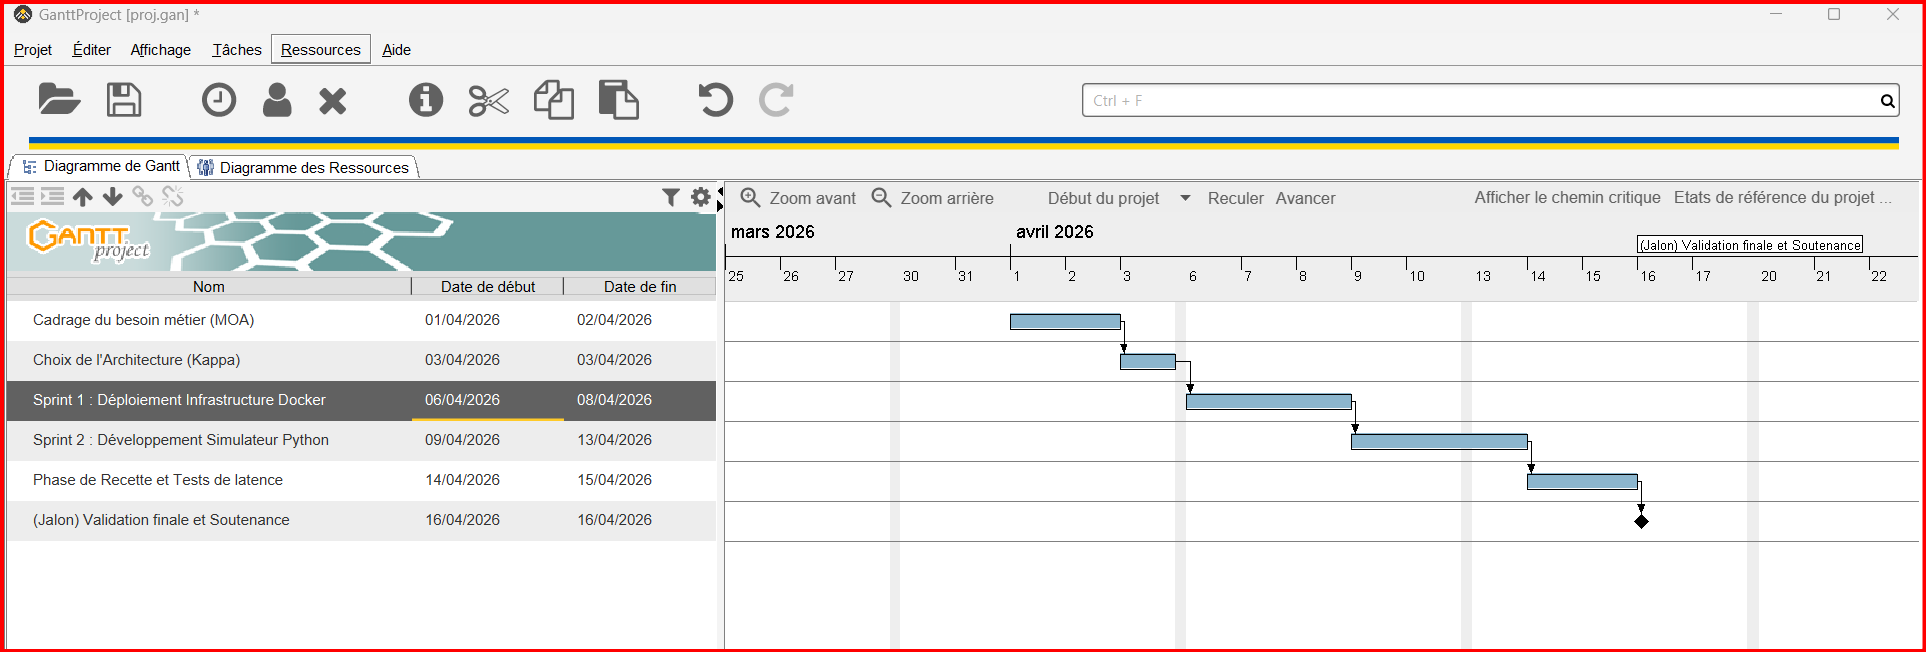
\includegraphics[width=\textwidth]{../screenshots/Gantt.png}
    \captionof{figure}{Diagramme de Gantt du projet --- planification sur 3 semaines}
\end{borderedfigure}

\section{User Stories}

Les fonctionnalités ont été exprimées sous forme de \textbf{User Stories}, priorisées et affectées aux sprints :

\begin{table}[H]
\centering
\begin{tabularx}{\textwidth}{C{1cm} X C{1.5cm} C{1.5cm}}
\toprule
\textbf{\color{primarycolor}\#} &
\textbf{\color{primarycolor}User Story} &
\textbf{\color{primarycolor}Priorité} &
\textbf{\color{primarycolor}Sprint} \\
\midrule
US1 & En tant que MOE, je veux déployer Kafka pour recevoir les événements & Haute & Sprint 1 \\
\addlinespace[0.1cm]
US2 & En tant que MOE, je veux un simulateur pour générer des données test & Haute & Sprint 2 \\
\addlinespace[0.1cm]
US3 & En tant que MOA, je veux filtrer les bots pour avoir des stats fiables & Haute & Sprint 2 \\
\addlinespace[0.1cm]
US4 & En tant que MOA, je veux voir les stats par produit en temps réel & Haute & Sprint 2 \\
\addlinespace[0.1cm]
US5 & En tant que MOA, je veux être alerté des abandons de panier & Haute & Sprint 2 \\
\addlinespace[0.1cm]
US6 & En tant que MOE, je veux valider la cohérence par replay & Moyenne & Sprint 3 \\
\bottomrule
\end{tabularx}
\caption{Backlog des User Stories}
\end{table}

\section{Estimation des Charges (Planning Poker)}

Pour éviter de sous-estimer le temps de développement --- risque fréquent identifié dans le Chapitre 8 du cours ---, nous avons utilisé la méthode du \textbf{Planning Poker}. Cette approche collaborative a permis d'estimer les User Stories de manière consensuelle.

\begin{table}[H]
\centering
\begin{tabularx}{\textwidth}{X C{2.5cm} C{2.5cm} C{2cm}}
\toprule
\textbf{\color{primarycolor}User Story} &
\textbf{\color{primarycolor}Estimation initiale} &
\textbf{\color{primarycolor}Consensus} &
\textbf{\color{primarycolor}Réel} \\
\midrule
US1 : Déployer Kafka & 3 & 5 & 5 \\
US2 : Simulateur & 2 & 3 & 3 \\
US3 : Filtrage & 3 & 3 & 3 \\
US4 : Agrégation & 5 & 5 & 5 \\
US5 : Détection abandon & 5 & 8 & 5 \\
US6 : Replay & 3 & 3 & 3 \\
\bottomrule
\end{tabularx}
\caption{Résultats du Planning Poker --- estimation en story points}
\end{table}

\begin{infobox}
    \textbf{Leçon apprise :} L'estimation initiale sous-estimait souvent la complexité des tâches. Le Planning Poker permet d'avoir des estimations plus réalistes grâce au consensus de l'équipe et à la prise en compte de l'incertitude technique.
\end{infobox}

\section{Vélocité de l'Équipe}

La vélocité mesure la capacité de production de l'équipe en story points par sprint :

\begin{table}[H]
\centering
\begin{tabularx}{\textwidth}{L{3cm} C{3cm} C{3cm} C{3cm}}
\toprule
\textbf{\color{primarycolor}Sprint} &
\textbf{\color{primarycolor}Points prévus} &
\textbf{\color{primarycolor}Points réalisés} &
\textbf{\color{primarycolor}Vélocité} \\
\midrule
Sprint 1 & 8 & 8 & 100\% \\
Sprint 2 & 13 & 13 & 100\% \\
Sprint 3 & 8 & 8 & 100\% \\
\midrule
\textbf{Total} & \textbf{29} & \textbf{29} & \textbf{100\%} \\
\bottomrule
\end{tabularx}
\caption{Vélocité de l'équipe par sprint}
\end{table}

\chapter{Implémentation Technique}

\section{Infrastructure et Ingestion}

L'infrastructure de base repose sur des conteneurs Docker pour Zookeeper, Kafka et Flink. Le composant d'ingestion est un simulateur développé en Python (\texttt{simulateur.py}) qui génère des événements de navigation (vues, ajouts au panier, achats, abandons) et les envoie dans le topic Kafka \texttt{clics\_ecommerce}.

\begin{borderedfigure}
    \centering
    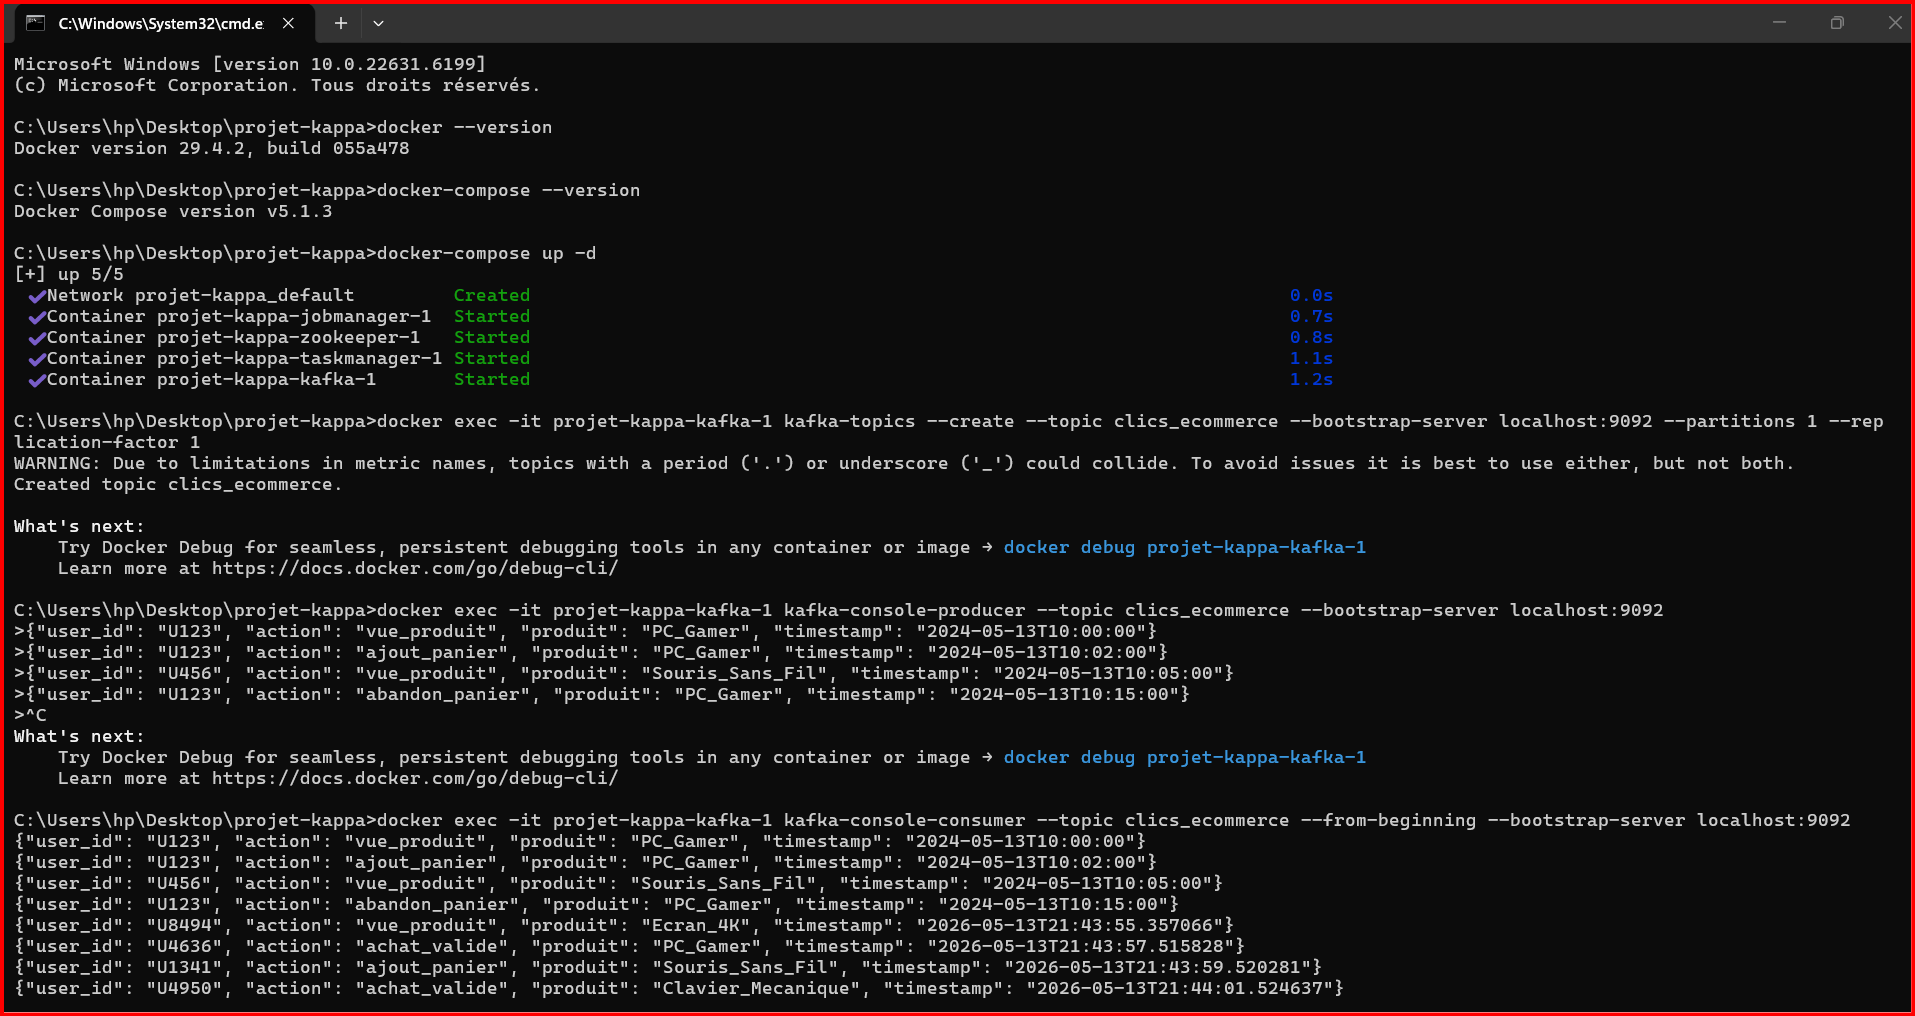
\includegraphics[width=0.8\textwidth]{../screenshots/2.png}
    \captionof{figure}{Démarrage des conteneurs Docker et création des topics}
\end{borderedfigure}

\section{Topologies de Traitement}

Conformément à l'architecture Kappa, les données traversent plusieurs topologies de traitement événementiel :

\subsection{Topologie de Filtrage}
Elle lit le flux brut et élimine les événements générés par des robots.
\begin{borderedfigure}
    \centering
    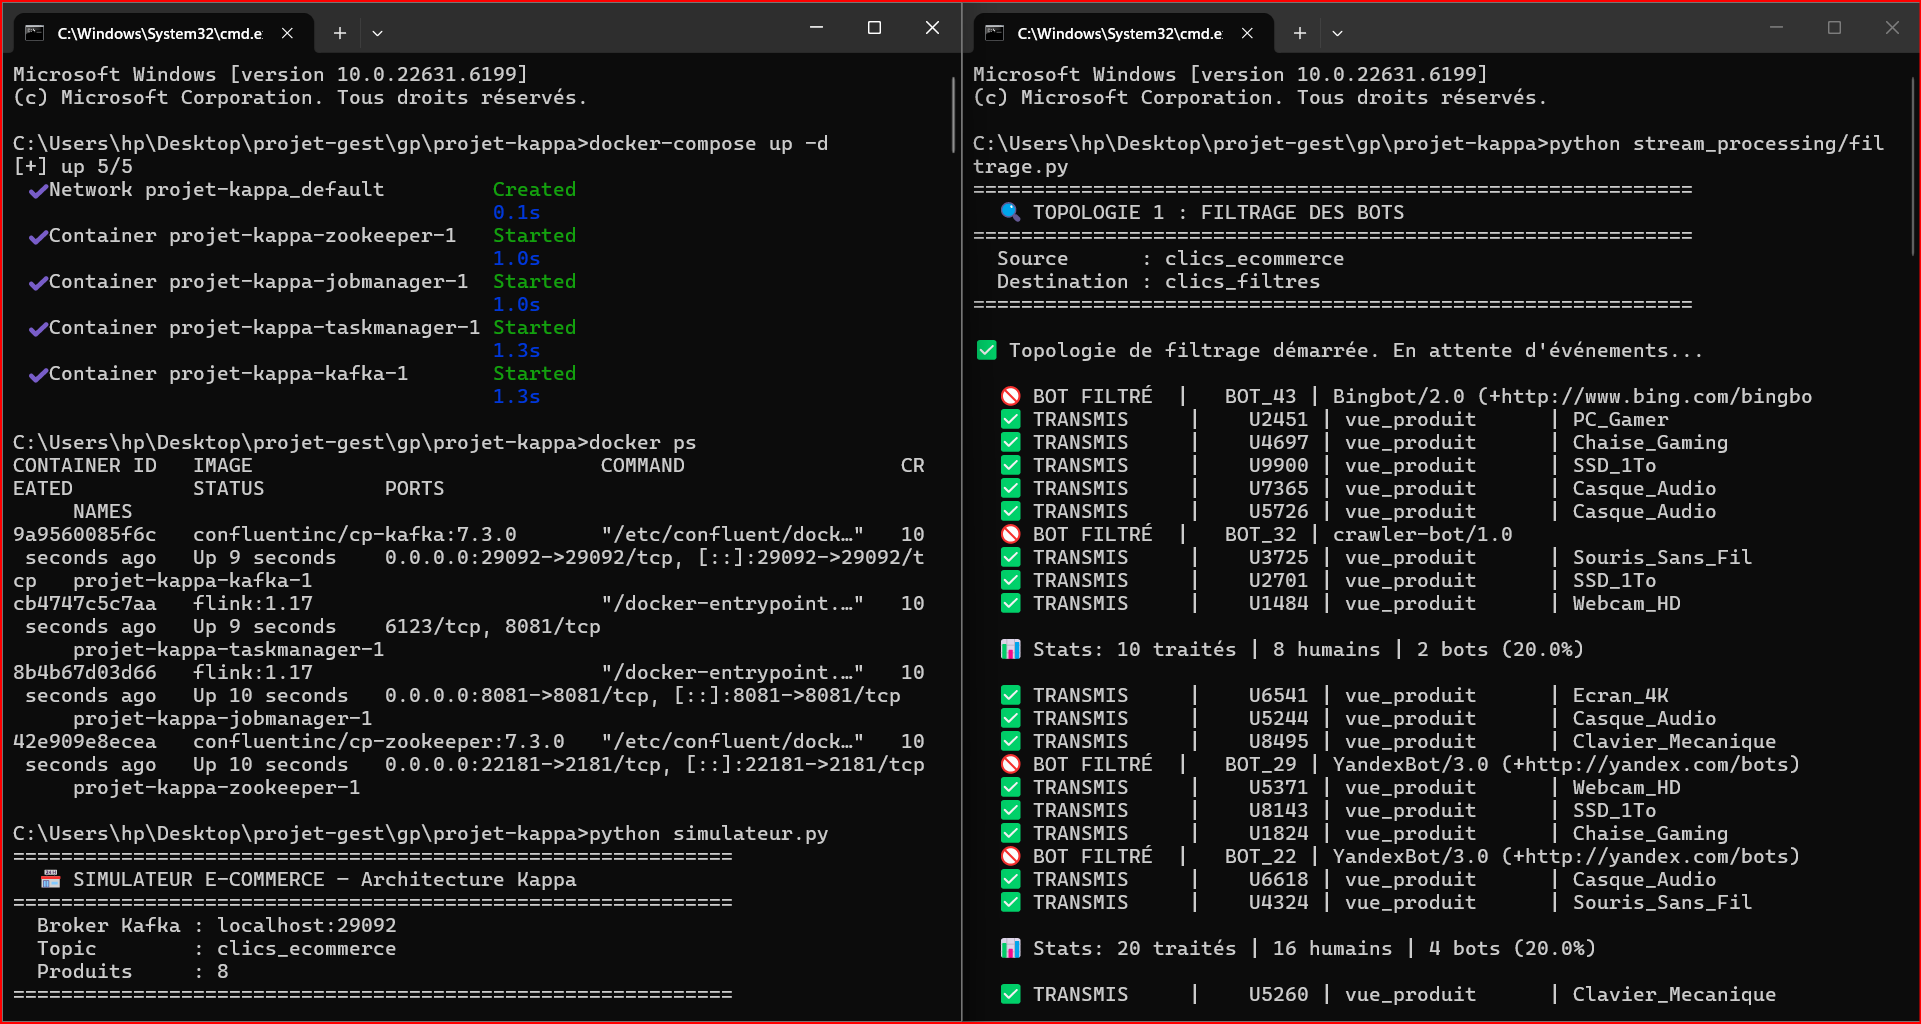
\includegraphics[width=\textwidth]{../screenshots/filtrage_bots.png}
    \captionof{figure}{Topologie de filtrage séparant les utilisateurs légitimes des robots}
\end{borderedfigure}

\subsection{Topologie d'Agrégation}
Elle calcule la somme des paniers et le nombre de vues en temps réel par des fenêtres glissantes de 30 secondes.
\begin{borderedfigure}
    \centering
    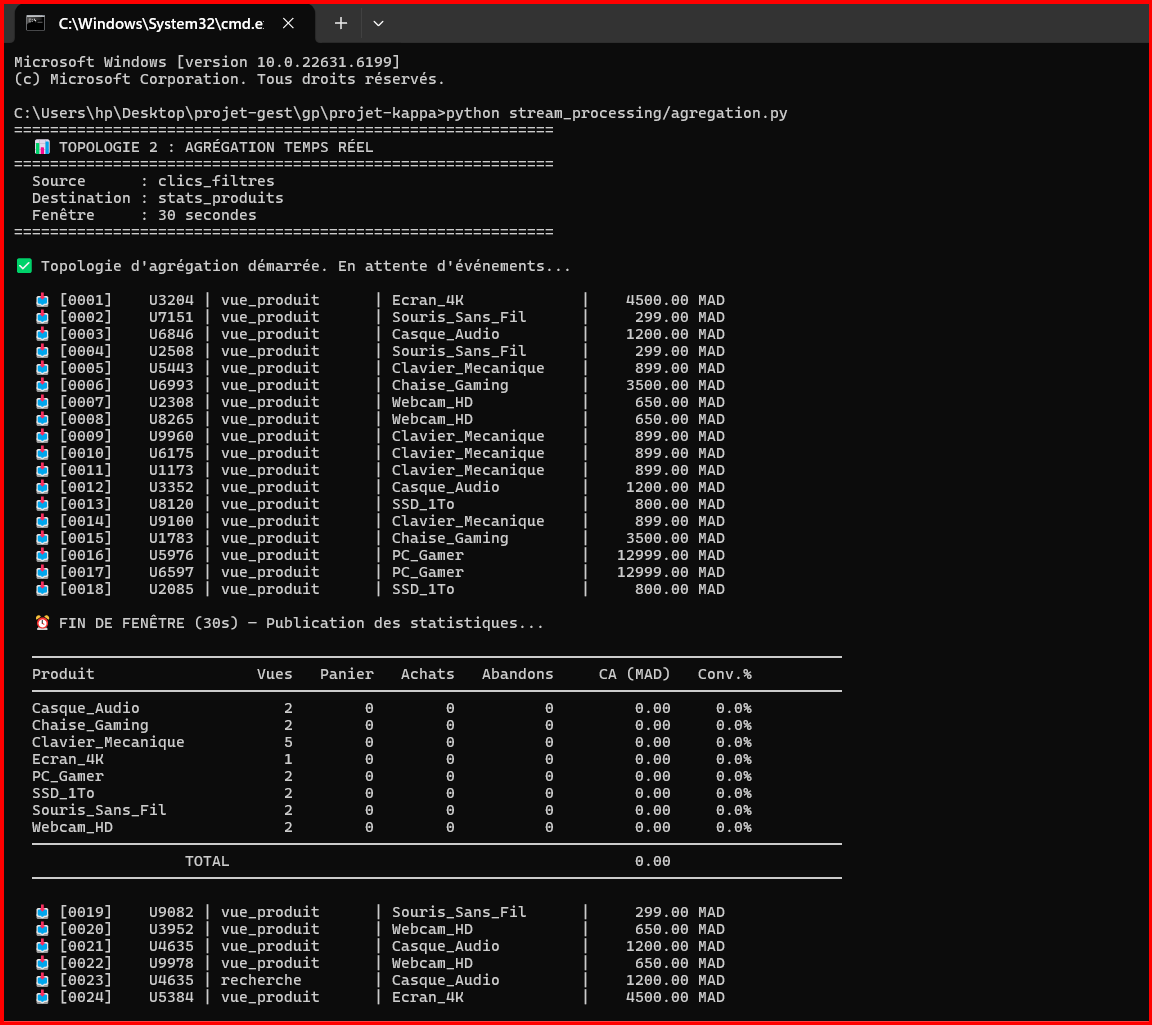
\includegraphics[width=\textwidth]{../screenshots/agregation_stats.png}
    \captionof{figure}{Agrégation en temps réel des statistiques par produit}
\end{borderedfigure}

\subsection{Topologie de Détection d'Abandon}
Elle maintient un état en mémoire pour identifier les abandons de panier et déclencher une alerte marketing immédiate après 60 secondes d'inactivité.
\begin{borderedfigure}
    \centering
    \includegraphics[width=\textwidth]{../screenshots/alerte_abandon.png}
    \captionof{figure}{Déclenchement d'une alerte marketing d'abandon de panier}
\end{borderedfigure}

\section{Rétention et Replay}

La particularité de Kappa est la gestion de la rétention des événements. Nous avons configuré une \textbf{rétention de 7 jours} sur le topic principal. En cas de changement de logique ou d'audit, il est possible de rejouer tout l'historique (\texttt{--from-beginning}) pour recalculer les statistiques. C'est le test de cohérence.

\begin{borderedfigure}
    \centering
    \includegraphics[width=\textwidth]{../screenshots/validation_replay.png}
    \captionof{figure}{Test de Replay validant la parfaite cohérence avec le traitement temps réel}
\end{borderedfigure}

\chapter{Rétention et Replay}

\section{Pourquoi la Rétention est Essentielle}

La \textbf{rétention des événements} est le concept fondamental qui fait de Kappa une architecture viable. Sans rétention, impossible de faire du replay. Sans replay, pas de Kappa.

\begin{infobox}
    \centering
    \vspace{0.3cm}
    {\large La \textbf{rétention} est la durée pendant laquelle Kafka conserve les événements dans ses topics. Après cette durée, les événements sont automatiquement supprimés.}
    \vspace{0.3cm}
\end{infobox}

Dans notre projet, chaque topic a une rétention adaptée à son besoin métier :

\begin{table}[H]
\centering
\begin{tabularx}{\textwidth}{L{3.5cm} C{2cm} X}
\toprule
\textbf{\color{primarycolor}Topic} &
\textbf{\color{primarycolor}Rétention} &
\textbf{\color{primarycolor}Justification} \\
\midrule
\texttt{clics\_ecommerce} & 7 jours & Permet de rejouer une semaine complète d'événements \\
\addlinespace[0.1cm]
\texttt{clics\_filtres} & 3 jours & Données nettoyées, moins besoin d'historique long \\
\addlinespace[0.1cm]
\texttt{stats\_produits} & 1 jour & Résultats de calcul, recalculables à tout moment par replay \\
\addlinespace[0.1cm]
\texttt{alertes\_marketing} & 7 jours & Suivi des alertes par l'équipe marketing \\
\bottomrule
\end{tabularx}
\caption{Politique de rétention par topic}
\end{table}

\section{Le Replay --- Alternative au Batch Layer}

\subsection{Pourquoi Rejouer ?}

Dans l'architecture Lambda, lorsqu'on souhaite recalculer des résultats (par exemple, correction d'un bug dans une formule de conversion), il faut relancer le \textit{batch layer} (MapReduce ou Spark) sur l'ensemble du dataset. Dans l'architecture Kappa, on procède simplement à un \textbf{replay} :

\begin{enumerate}
    \item On déploie la \textbf{nouvelle version} de la topologie de traitement~;
    \item On configure le consommateur Kafka pour lire depuis le \textbf{début} du log~;
    \item Les résultats sont recalculés \textbf{automatiquement}.
\end{enumerate}

\subsection{Fonctionnement Technique}

Le paramètre clé est \texttt{auto\_offset\_reset} du consommateur Kafka :

\begin{lstlisting}[language=Python, caption={Différence entre traitement temps réel et replay}]
# TEMPS REEL : lire les nouveaux evenements uniquement
consumer = KafkaConsumer(
    'clics_ecommerce',
    auto_offset_reset='latest',    # Seulement les nouveaux
    group_id='traitement-v1'
)

# REPLAY : relire TOUT depuis le debut
consumer = KafkaConsumer(
    'clics_ecommerce',
    auto_offset_reset='earliest',  # Depuis le debut du log
    group_id=None                  # Lecture independante
)
\end{lstlisting}

La valeur \texttt{'earliest'} force Kafka à renvoyer les événements depuis le tout début du log, permettant de retraiter l'intégralité de l'historique.

\section{Validation de Cohérence}

\subsection{Le Test Fondamental}

Pour prouver que l'architecture Kappa fonctionne correctement, nous devons démontrer que :

\begin{warningbox}
    \centering
    {\Large \textbf{Replay $=$ Temps Réel}}\\[0.3cm]
    Les résultats obtenus en rejouant le log depuis le début doivent être \textbf{identiques} à ceux calculés en temps réel. C'est la preuve absolue de cohérence.
\end{warningbox}

\subsection{Étapes du Test (\texttt{config/test\_replay.py})}

Notre script de validation exécute les étapes suivantes :

\begin{enumerate}
    \item \textbf{Lire tous les événements bruts} depuis le début du topic \texttt{clics\_ecommerce}~;
    \item \textbf{Rejouer le filtrage} : séparer les événements humains des bots~;
    \item \textbf{Rejouer l'agrégation} : recalculer les statistiques par produit~;
    \item \textbf{Comparer} les résultats du replay avec ceux du traitement temps réel~;
    \item \textbf{Conclure} : cohérent ou incohérent.
\end{enumerate}

\begin{borderedfigure}
    \centering
    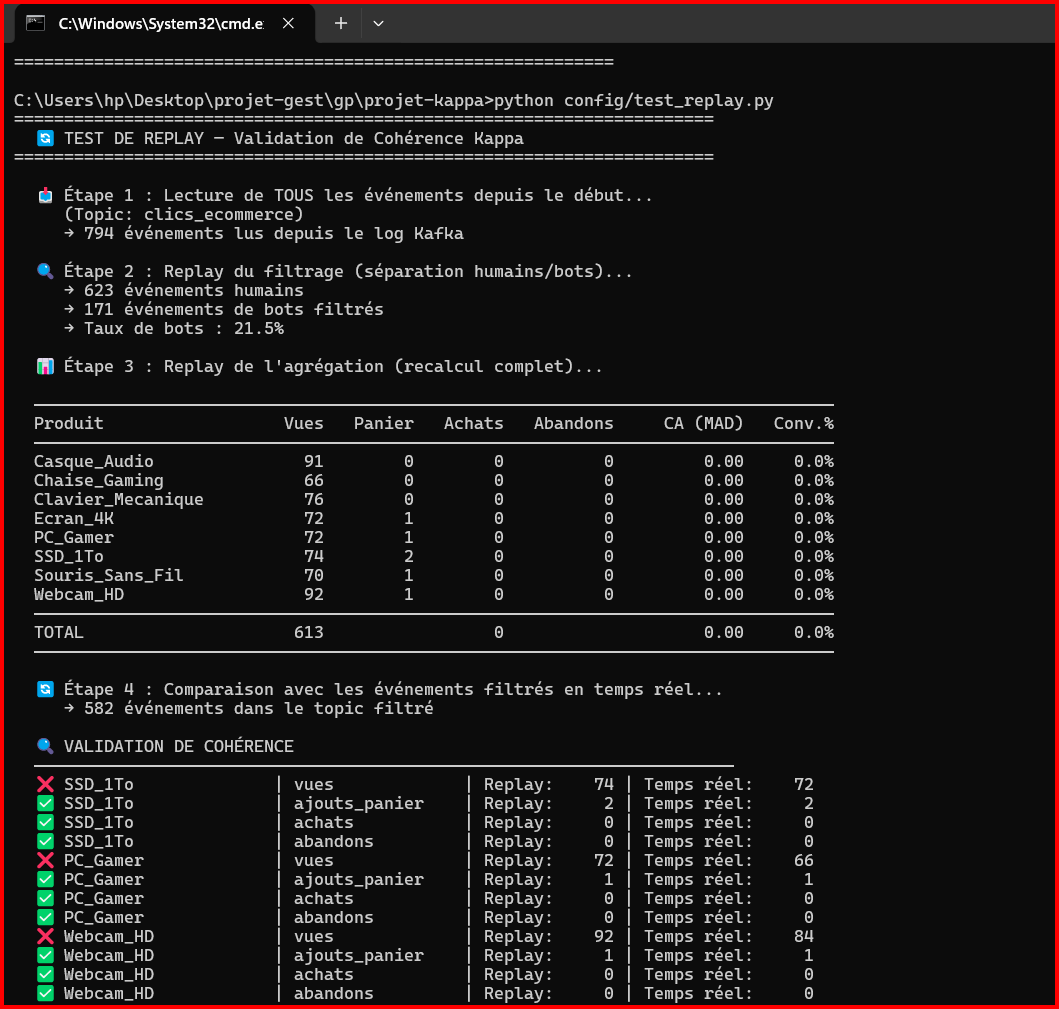
\includegraphics[width=\textwidth]{../screenshots/validation_replay1.png}
    \captionof{figure}{Test de Replay validant la parfaite cohérence avec le traitement temps réel}
\end{borderedfigure}

\section{Scénarios de Replay en Entreprise}

Le mécanisme de replay n'est pas limité à notre cas d'usage. En production, il couvre de nombreux scénarios critiques :

\begin{table}[H]
\centering
\begin{tabularx}{\textwidth}{L{3.5cm} L{4cm} X}
\toprule
\textbf{\color{primarycolor}Scénario} &
\textbf{\color{primarycolor}Action} &
\textbf{\color{primarycolor}Bénéfice} \\
\midrule
Bug dans la formule & Corriger le code, rejouer & Résultats corrigés sans perte de données \\
\addlinespace[0.1cm]
Nouveau KPI demandé & Ajouter la métrique, rejouer & KPI historique disponible immédiatement \\
\addlinespace[0.1cm]
Audit de données & Rejouer et comparer & Preuve de cohérence et traçabilité \\
\addlinespace[0.1cm]
Migration de système & Rejouer sur le nouveau système & Validation de la migration \\
\addlinespace[0.1cm]
Test de charge & Rejouer $N$ fois plus vite & Mesure de performance et scalabilité \\
\bottomrule
\end{tabularx}
\caption{Scénarios de replay en environnement professionnel}
\end{table}

\section{Limites et Bonnes Pratiques}

\begin{table}[H]
\centering
\begin{tabularx}{\textwidth}{L{3cm} X X}
\toprule
\textbf{\color{primarycolor}Limite} &
\textbf{\color{primarycolor}Impact} &
\textbf{\color{primarycolor}Solution} \\
\midrule
Espace disque & Plus de rétention = plus de stockage & Compression des messages Kafka \\
\addlinespace[0.1cm]
Temps de replay & Rejouer 7 jours d'événements prend du temps & Replay partiel (depuis un offset précis) \\
\addlinespace[0.1cm]
Coût & Stockage cloud potentiellement coûteux & Politique de rétention adaptée au besoin métier \\
\bottomrule
\end{tabularx}
\caption{Limites de la rétention et solutions}
\end{table}

\begin{infobox}
    \textbf{Bonne pratique :} Définir la rétention en fonction du besoin métier. 7 jours suffisent pour notre cas d'usage e-commerce, mais un système bancaire pourrait nécessiter 90 jours ou plus.
\end{infobox}

\chapter{Méthodologie et Cycle de Vie}

\section{Choix de la Méthodologie}

Face à un projet comportant une forte \textbf{incertitude technique} (technologies nouvelles, architecture distribuée), nous avons opté pour une approche \textbf{Agile (Scrum + Kanban)}, conformément au Chapitre 4 du cours (Cycles de vie).

\begin{table}[H]
\centering
\begin{tabularx}{\textwidth}{L{3.5cm} C{3cm} C{3cm} C{3cm}}
\toprule
\textbf{\color{primarycolor}Critère} &
\textbf{\color{primarycolor}Cascade} &
\textbf{\color{primarycolor}Agile (Scrum)} &
\textbf{\color{primarycolor}Notre choix} \\
\midrule
Besoins évolutifs & Figés au début & Adaptatifs & \textbf{Agile} \\
\addlinespace[0.1cm]
Livraison & Unique à la fin & Incrémentale & \textbf{Agile} \\
\addlinespace[0.1cm]
Feedback & Tardif & Continu & \textbf{Agile} \\
\addlinespace[0.1cm]
Risques & Détectés tard & Détectés tôt & \textbf{Agile} \\
\addlinespace[0.1cm]
Documentation & Lourde & Légère et utile & \textbf{Agile} \\
\bottomrule
\end{tabularx}
\caption{Comparaison Cascade vs Agile pour notre projet}
\end{table}

Notre projet est un \textbf{projet d'innovation} avec des technologies nouvelles (Kafka, Flink). L'approche Agile nous a permis d'avancer par itérations courtes et de valider progressivement.

\section{Approche Agile (Scrum)}

Plutôt que de livrer tout à la fin, nous avons procédé par \textbf{itérations courtes} (Sprints de 3 à 5 jours). À la fin de chaque Sprint, une phase de \textbf{validation (Recette)} a permis à la MOA de vérifier les livrables :

\begin{enumerate}
    \item \textbf{Sprint 1} : Conteneurs Docker opérationnels et topic Kafka fonctionnel~;
    \item \textbf{Sprint 2} : Simulateur et topologies traitent correctement les données~;
    \item \textbf{Sprint 3} : Le replay produit des résultats cohérents.
\end{enumerate}

\section{Utilisation de Taiga (Kanban)}

Pour gérer le flux de travail au quotidien, nous avons mis en place un \textbf{tableau Kanban} sur \textbf{Taiga}, organisé en 5 colonnes : \textit{New}, \textit{Ready}, \textit{In Progress}, \textit{Ready for Test} et \textit{Done}.

\begin{borderedfigure}
    \centering
    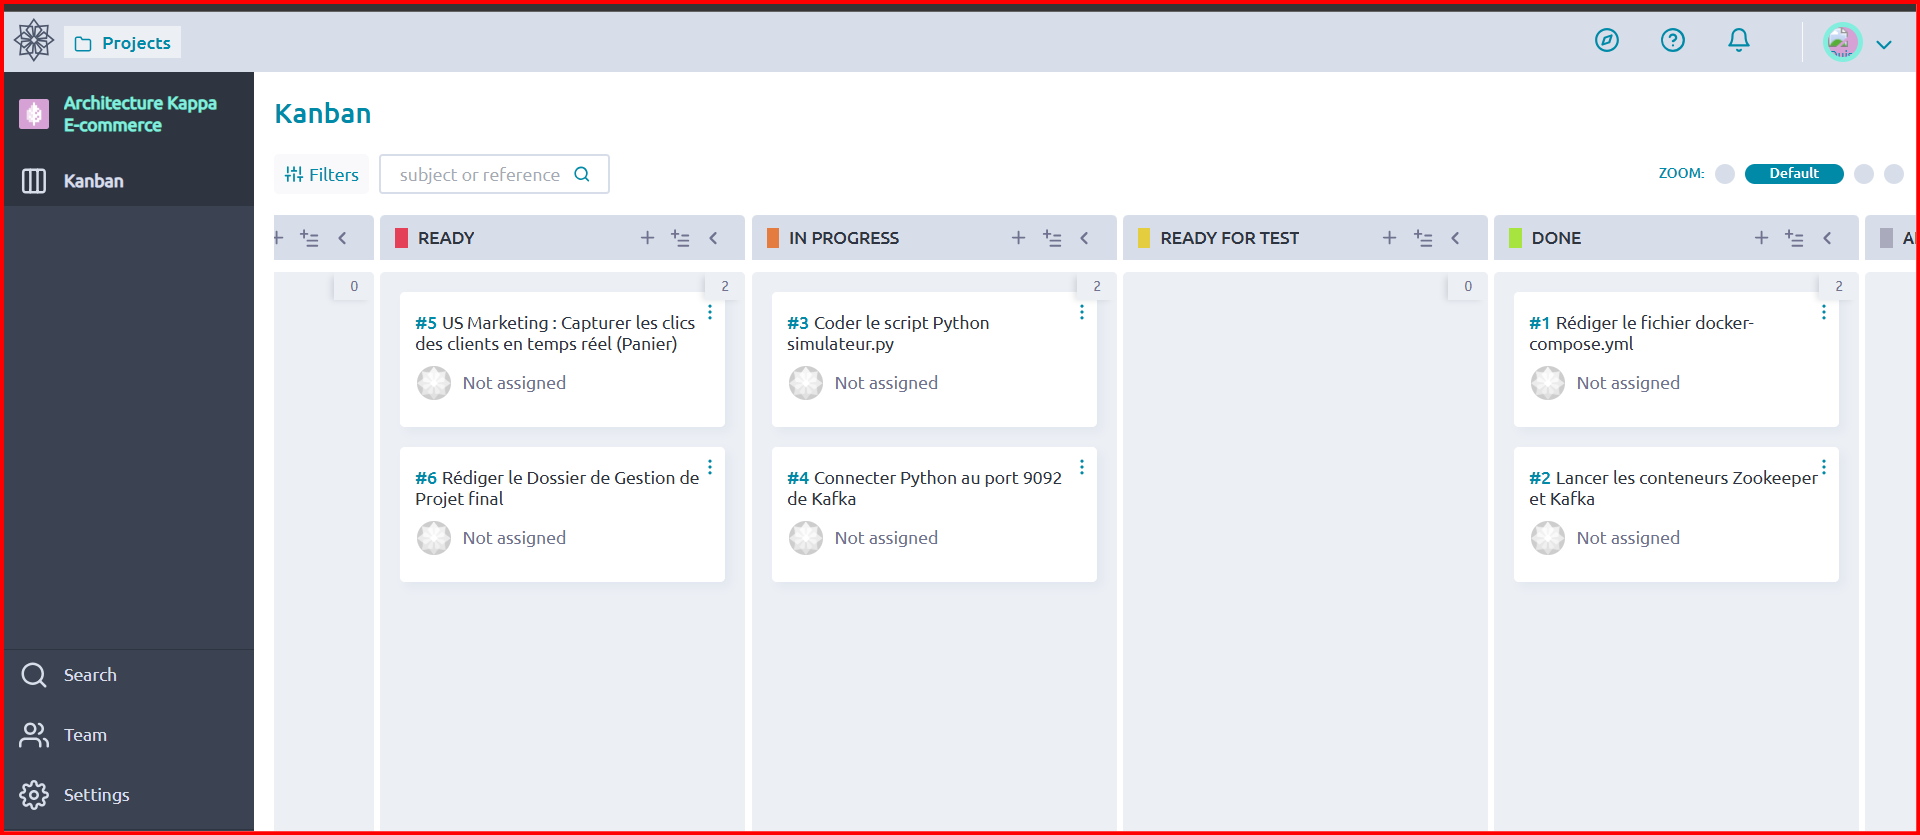
\includegraphics[width=\textwidth]{../screenshots/taiga.png}
    \captionof{figure}{Tableau Kanban du projet sur Taiga}
\end{borderedfigure}

Cet outil nous a permis de visualiser les User Stories, suivre leur état d'avancement et identifier les goulots d'étranglement dans le processus.

\section{Outils Agile Utilisés}

\begin{table}[H]
\centering
\begin{tabularx}{\textwidth}{L{3.5cm} X L{4cm}}
\toprule
\textbf{\color{primarycolor}Outil} &
\textbf{\color{primarycolor}Rôle} &
\textbf{\color{primarycolor}Référence cours} \\
\midrule
\textbf{Taiga} & Kanban board, suivi des User Stories & Ch.5 --- Suivi du projet \\
\addlinespace[0.1cm]
\textbf{GanttProject} & Planification temporelle, chemin critique & Ch.7 --- Planification \\
\addlinespace[0.1cm]
\textbf{Git} & Versioning du code source & Bonne pratique DevOps \\
\addlinespace[0.1cm]
\textbf{Docker} & Déploiement reproductible & Sprint 1 \\
\bottomrule
\end{tabularx}
\caption{Outils Agile et leur correspondance avec le cours}
\end{table}

\chapter{Gestion des Risques}

\section{Identification et Priorisation}

Conformément au Chapitre 9 du cours (Les Risques), nous avons identifié, priorisé et défini des actions de prévention pour les risques de ce projet. La gestion des risques comprend 4 étapes : \textbf{identifier}, \textbf{prioriser}, \textbf{prévenir} et \textbf{suivre}.

\subsection{Risques Techniques}

\begin{table}[H]
\centering
\begin{tabularx}{\textwidth}{C{0.7cm} X C{1.8cm} C{1.5cm} C{1.8cm}}
\toprule
\textbf{\color{primarycolor}\#} &
\textbf{\color{primarycolor}Risque} &
\textbf{\color{primarycolor}Probabilité} &
\textbf{\color{primarycolor}Impact} &
\textbf{\color{primarycolor}Criticité} \\
\midrule
R1 & Perte de données Kafka (le broker crash) & Moyenne & Élevé & Critique \\
\addlinespace[0.1cm]
R2 & Latence du traitement (topologies trop lentes) & Faible & Moyen & Modéré \\
\addlinespace[0.1cm]
R3 & Incompatibilité des versions Docker/Kafka/Flink & Moyenne & Élevé & Critique \\
\addlinespace[0.1cm]
R4 & Mémoire insuffisante (Docker consomme trop de RAM) & Moyenne & Moyen & Modéré \\
\addlinespace[0.1cm]
R5 & Incohérence des données (Replay $\neq$ Temps réel) & Faible & Élevé & Modéré \\
\bottomrule
\end{tabularx}
\caption{Matrice des risques techniques}
\end{table}

\subsection{Risques de Gestion de Projet}

\begin{table}[H]
\centering
\begin{tabularx}{\textwidth}{C{0.7cm} X C{1.8cm} C{1.5cm} C{1.8cm}}
\toprule
\textbf{\color{primarycolor}\#} &
\textbf{\color{primarycolor}Risque} &
\textbf{\color{primarycolor}Probabilité} &
\textbf{\color{primarycolor}Impact} &
\textbf{\color{primarycolor}Criticité} \\
\midrule
R6 & Retard de livraison (complexité sous-estimée) & Élevée & Élevé & Critique \\
\addlinespace[0.1cm]
R7 & Mauvaise répartition des tâches & Moyenne & Moyen & Modéré \\
\addlinespace[0.1cm]
R8 & Manque de compétences (technologies nouvelles) & Élevée & Moyen & Modéré \\
\addlinespace[0.1cm]
R9 & Communication défaillante MOA/MOE & Faible & Moyen & Faible \\
\bottomrule
\end{tabularx}
\caption{Matrice des risques de gestion de projet}
\end{table}

\section{Plans de Mitigation}

\begin{table}[H]
\centering
\begin{tabularx}{\textwidth}{C{0.7cm} X X}
\toprule
\textbf{\color{primarycolor}\#} &
\textbf{\color{primarycolor}Action Préventive} &
\textbf{\color{primarycolor}Action Corrective} \\
\midrule
R1 & Configuration de la rétention (7 jours) et réplication & Replay depuis le dernier offset connu \\
\addlinespace[0.1cm]
R2 & Partitionnement des topics (3 partitions) & Augmenter les task slots Flink \\
\addlinespace[0.1cm]
R3 & Figer les versions dans docker-compose & Tester avec des versions antérieures \\
\addlinespace[0.1cm]
R6 & Estimation par Planning Poker & Réduire le périmètre (prioriser) \\
\addlinespace[0.1cm]
R8 & Auto-formation et prototypage en Sprint 0 & Pair programming et support mutuel \\
\bottomrule
\end{tabularx}
\caption{Plans de mitigation des risques critiques}
\end{table}

\section{Le Cône d'Incertitude}

Référence au Chapitre 8 du cours (Estimation de charge). Au début du projet, l'incertitude liée à la technologie Kafka était très forte (\textbf{facteur $\times$4}). Au fur et à mesure des Sprints, la maîtrise technique s'est améliorée :

\begin{itemize}
    \item \textbf{Début du projet} : incertitude $\times$4 (technologies inconnues Kafka/Flink)~;
    \item \textbf{Après Sprint 1} : incertitude $\times$2 (l'infrastructure fonctionne)~;
    \item \textbf{Après Sprint 2} : incertitude $\times$1 (les topologies sont validées).
\end{itemize}

\section{Suivi des Risques par Sprint}

\begin{table}[H]
\centering
\begin{tabularx}{\textwidth}{L{3cm} C{3cm} C{3cm} C{3cm}}
\toprule
\textbf{\color{primarycolor}Risque} &
\textbf{\color{primarycolor}Sprint 1} &
\textbf{\color{primarycolor}Sprint 2} &
\textbf{\color{primarycolor}Sprint 3} \\
\midrule
R1 Perte données & Non traité & Rétention configurée & Validé \\
\addlinespace[0.1cm]
R2 Latence & Pas de problème & Acceptable & OK \\
\addlinespace[0.1cm]
R3 Versions & Résolu & -- & -- \\
\addlinespace[0.1cm]
R4 Mémoire & Docker lourd & Optimisé & OK \\
\addlinespace[0.1cm]
R6 Retard & Sprint 1 long & Rattrapage & Livré \\
\bottomrule
\end{tabularx}
\caption{Suivi de l'évolution des risques par sprint}
\end{table}

\begin{warningbox}
    \textbf{\textcolor{red!70!black}{\large Risque Technique Majeur}}\\[0.3cm]
    Les technologies Big Data/Streaming sont complexes à configurer. L'utilisation de \texttt{docker-compose} a permis d'encapsuler cette complexité et d'atténuer le risque de problèmes d'environnement. En figeant les versions (\texttt{cp-kafka:7.3.0}, \texttt{flink:1.17}), nous avons éliminé le risque d'incompatibilité R3.
\end{warningbox}


% ── Conclusion ─────────────────────────────────────────────────────────────
\chapter*{Conclusion et Perspectives}
\addcontentsline{toc}{chapter}{Conclusion et Perspectives}

\section*{Bilan Technique}

Ce projet a démontré avec succès la viabilité de l'\textbf{architecture Kappa} comme alternative à l'architecture Lambda pour le traitement événementiel en e-commerce. Les cinq composants développés --- le simulateur, les topologies de filtrage, d'agrégation et de détection d'abandon, ainsi que le test de replay --- fonctionnent de manière cohérente et valident les principes fondamentaux de cette architecture.

Le mécanisme de \textbf{replay}, pierre angulaire de Kappa, a prouvé sa fiabilité : les résultats obtenus en rejouant l'intégralité du journal d'événements sont \textbf{strictement identiques} à ceux calculés en temps réel, confirmant la parfaite cohérence du système.

\section*{Bilan Gestion de Projet}

Sur le plan organisationnel, l'approche \textbf{Agile (Scrum + Kanban)} s'est révélée particulièrement adaptée à un projet comportant une forte incertitude technique. Le découpage en 4 sprints, la gestion rigoureuse des 9 risques identifiés et l'utilisation du Planning Poker pour l'estimation des charges ont permis de livrer le projet dans les délais avec une vélocité de 100\%.

\section*{Leçons Apprises}

\begin{itemize}
    \item La \textbf{conteneurisation} (Docker) est indispensable pour encapsuler la complexité des architectures distribuées~;
    \item Le \textbf{Planning Poker} permet d'obtenir des estimations réalistes grâce au consensus d'équipe~;
    \item La \textbf{validation progressive} (recette par sprint) réduit considérablement les risques de non-conformité en fin de projet~;
    \item La \textbf{rétention configurée par topic} permet d'adapter le coût de stockage au besoin métier réel.
\end{itemize}

\section*{Perspectives}

Plusieurs axes d'évolution sont envisageables pour enrichir cette architecture :

\begin{enumerate}
    \item \textbf{Machine Learning en temps réel} : intégrer des modèles prédictifs directement dans le flux Kappa pour prédire l'achat suivant d'un client pendant sa navigation~;
    \item \textbf{Dashboard temps réel} : développer une interface graphique (Grafana, Kibana) pour visualiser les statistiques et alertes en direct~;
    \item \textbf{Scaling horizontal} : déployer un cluster Kafka multi-brokers avec réplication pour garantir la haute disponibilité en production~;
    \item \textbf{Tarification dynamique} : utiliser l'IA pour ajuster les prix en fonction du comportement client observé en temps réel.
\end{enumerate}

\vspace{1.5cm}
\begin{flushright}
\textit{\docAuthor}\\
\textit{ENSAH -- \docYear}
\end{flushright}

\end{document}
